
%(BEGIN_QUESTION)
% Copyright 2011, Tony R. Kuphaldt, released under the Creative Commons Attribution License (v 1.0)
% This means you may do almost anything with this work of mine, so long as you give me proper credit

Anta at følgende reguleringssystem fungerer som designet under normal drift (dvs. skorsteinstemperatur 1550 $^{o}$F). Metalltemperaturen holdes nøyaktig på settpunktet 1425 $^{o}$F:

$$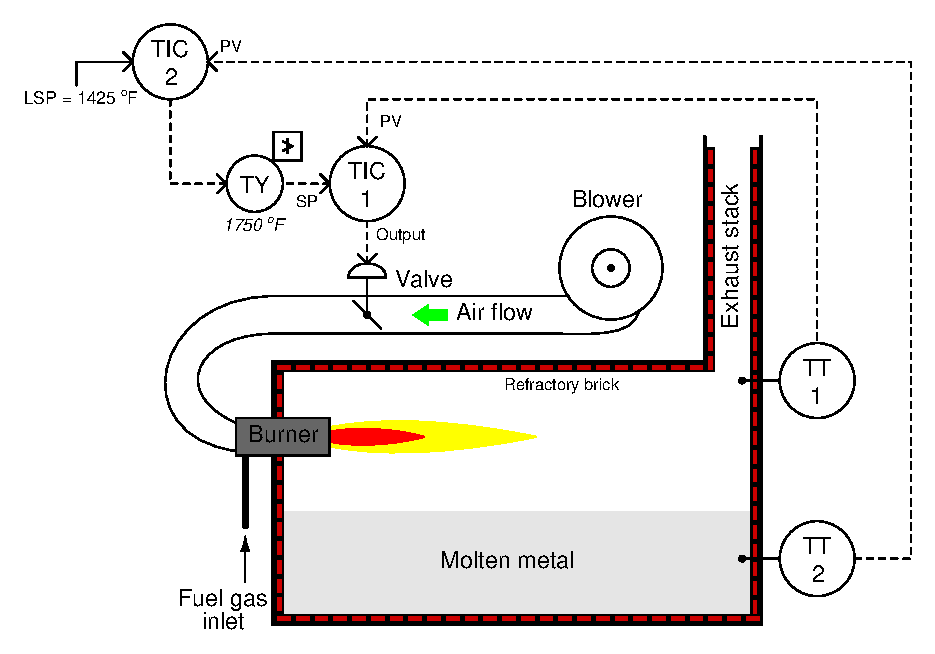
\includegraphics[width=15.5cm]{i03091x01.eps}$$

\noindent
Velg beste svar som beskriver umiddelbar prosesseffekt hvis temperaturtransmitter TT-2 plutselig feiler med {\it høyt} signal:

\begin{itemize}
\item{} Skorsteinstemperaturen begynner å stige fordi regulatoren krever mer varme
\vskip 10pt
\item{} Begrensningsreleet (TY) overstyrer utgangssignalet fra TIC-2
\vskip 10pt
\item{} Systemet fortsetter normal drift og holder temperaturene stabile
\vskip 10pt
\item{} Ventilen begynner plutselig å stenge, og varmeinnmatingen til ovnen reduseres
\end{itemize}

\underbar{file i00875}
%(END_QUESTION)





%(BEGIN_ANSWER)

Ventilen begynner plutselig å stenge, og varmeinnmatingen til ovnen reduseres

%(END_ANSWER)





%(BEGIN_NOTES)

{\bf Denne oppgaven er ment kun for eksamen, ikke for arbeidsark!}.

%(END_NOTES)
